%\subsection{Pseudoscalar}
In this section, we check the consistency of the \hdma model as a function of the parameters chosen for the scans with the measured DM relic density, according to the standard thermal relic "freeze-out" scenario. This exercise requires the following assumptions, already described in Ref.~\cite{Albert:2017onk}: 

\begin{itemize}
\item The DM annihilation cross section receives only contributions from the interactions of the simplified model, while possible additional degrees of freedom and couplings not included in the model are irrelevant.
\item The DM number density in the Universe today is entirely determined by the DM annihilation cross section predicted by the \hdma. In particular, no additional mechanisms exist that enhance or deplete the relic density. 
\end{itemize}

It it important to realize that if one or both of these assumptions are violated there is no strict correlation between the relic density and the strength of mono-X signals. For instance, if DM is overproduced, the relic density can be reduced if the DM has large annihilation cross sections to new hidden sector states. These states might however not be directly accessible at LHC energies. Conversely, the correct DM relic density can still be obtained if the DM is underproduced. For instance, if the hidden sector carries an particle-antiparticle asymmetry (similar to the baryon asymmetry) then this necessarily leads to a larger relic density compared to the conventional freeze-out picture.

\subsection{Technical setup}

\begin{figure}[h]
\centering
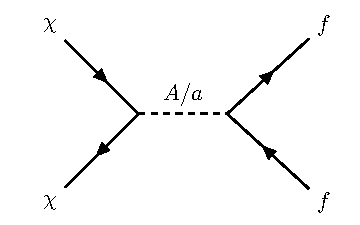
\includegraphics[width=0.35\textwidth]{texinputs/05_relic/figures/feynman/graph_2hdm_relic_s_fermions.pdf}
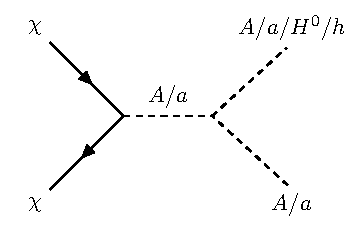
\includegraphics[width=0.35\textwidth]{texinputs/05_relic/figures/feynman/graph_2hdm_relic_s_bosons.pdf}
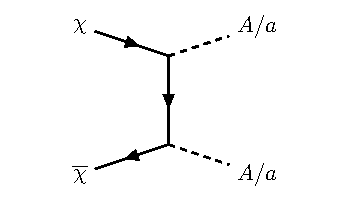
\includegraphics[width=0.35\textwidth]{texinputs/05_relic/figures/feynman/graph_2hdm_relic_ss_bosons.pdf}
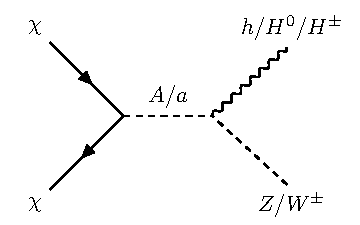
\includegraphics[width=0.35\textwidth]{texinputs/05_relic/figures/feynman/graph_2hdm_relic_s_vbosons.pdf}

\caption{Annihilation diagrams taken into account in the relic density calculation.}
\label{fig:feyn_annihilation}
\end{figure}

The \maddm~\cite{Backovic:2013dpa,Backovic:2015cra} plugin for \mgamcnlo is used to calculate the present-day relic density for this model.
%By modeling the thermal evolution of the cross-section during the expansion of the early universe, the time of freeze-out is determined.
All tree-level annihilation processes are taken into account, and the Yukawa couplings of all fermions are taken to be non-zero.
The Feynman diagrams of annihilation processes taken into account in this calculation are shown in \autoref{fig:feyn_annihilation}. Generally, the annihilation proceeds via single or double s-channel exchange of the pseudoscalars $a$ and $A$, with subsequent decays. Since \maddm uses only tree-level diagrams, contributions from off-shell pseudoscalars can only be taken into account for the case of single s-channel mediation with direct decay of the pseudoscalars to SM fermions. If the pseudoscalars instead decays to other bosons or if the annihilation proceeds through double s-channel diagrams, the outgoing bosons are taken to be on-shell and their decays are not simulated. 

Following \autoref{sec:ParameterScan}, we use the parameter choices $sin(\theta)=0.35$, $m_{h} = 125 GeV$, $g_{\chi}=1$, $\lambda_i = 3$ for all scans in this section.

\subsection{Results}

\begin{figure}[h]
\centering
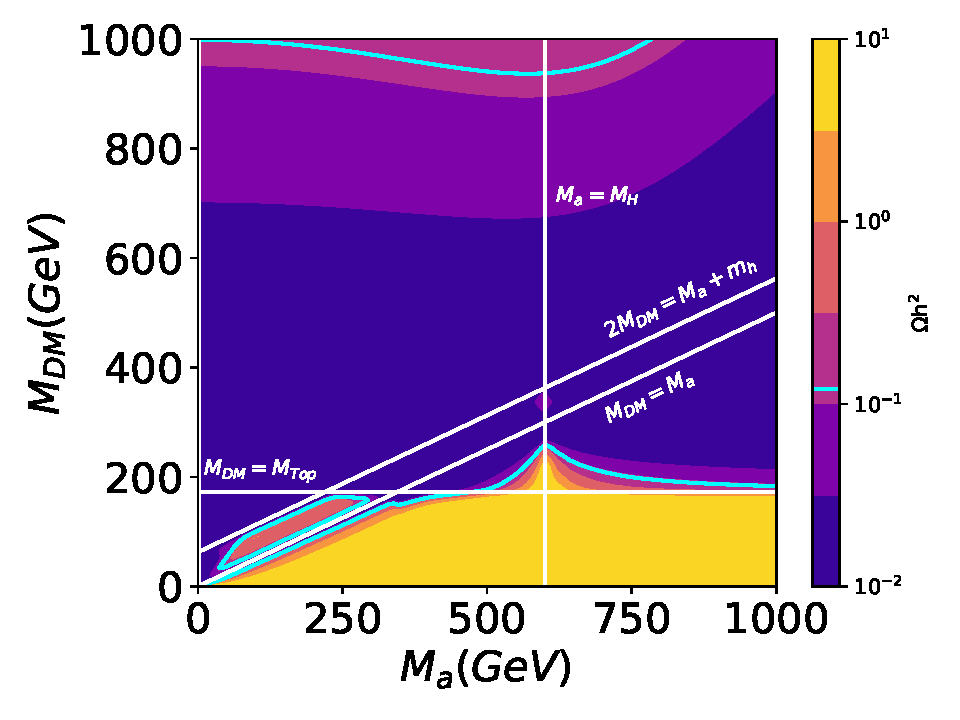
\includegraphics[width=0.49\textwidth]{{texinputs/05_relic/figures/relic/contour_scan_mxd_ma.pdf}}
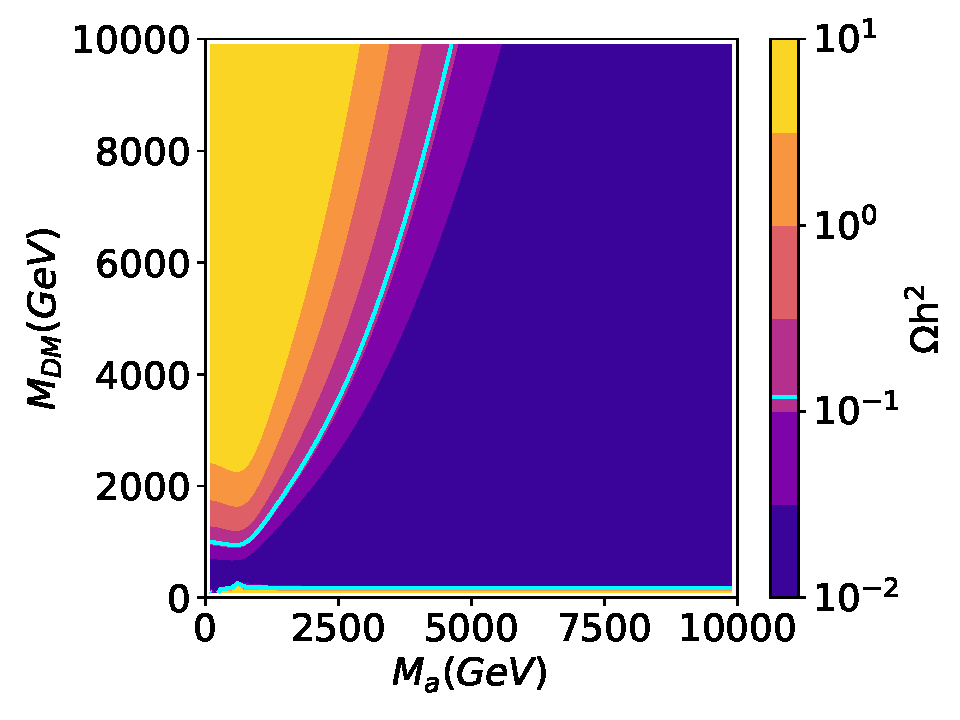
\includegraphics[width=0.49\textwidth]{{texinputs/05_relic/figures/relic/contour_scan_mxd_ma_large.pdf}}
\caption{Predicted relic density for a two-dimensional scan of \mDM and \ma. The other parameters of the model remain fixed with $m_{H}=m_{A}=m_{H^{\pm}}=\unit[600]{GeV}$ and $\tanb=1$, as well as the default choices described in the text. The color scale indicates the relic density, the cyan solid line shows the observed value of $\Omega h^{2} = 0.12$. The color scale is truncated at its ends, i.e. values larger than the maximum or smaller than the minimum are shown in the same color as the maximum/minimum. While the left focuses on the mass region relevant to collider searches, the right panel shows the development of the relic density for a larger mass region.}
\label{fig:relic_scan_mxd_ma}
\end{figure}

The relic density is shown for in the \ma-\mDM plane in \autoref{fig:relic_scan_mxd_ma}.
For small values of $\mDM$ below the mass of the top quark, DM is mostly overabundant. 
In this regime, annihilation to quarks is suppressed by the small Yukawa couplings of the light fermions. 
The observed relic density can only be achieved for $\mDM\approx\ma/2$, where annihilation is resonantly enhanced, or for $\mDM \approx (\ma+\mh)/2$, close to the threshold for the $\chi\chi\rightarrow h a$ process.
Above the top threshold, annihilation into fermions becomes very efficient and DM is underabundant. 
As \mDM increases further, annihilation via single s-channel diagrams is increasingly suppressed and the relic density rises again. 
The observed density is produced by this model for $\mDM\approx1 \mathrm{TeV}$ at low \ma.
\textbf{[The following sentence is being checked with Andreas Albert - would remove]} For values of \ma beyond the LHC reach of a few TeV, the allowed parameter region at the top threshold $\mDM\approx m_{\mathrm{top}}$ remains independent of the value of \ma, indicating that a DM candidate that is mass degenerate with the top quark cannot be excluded by LHC searches alone.

\begin{figure}[h]
\centering
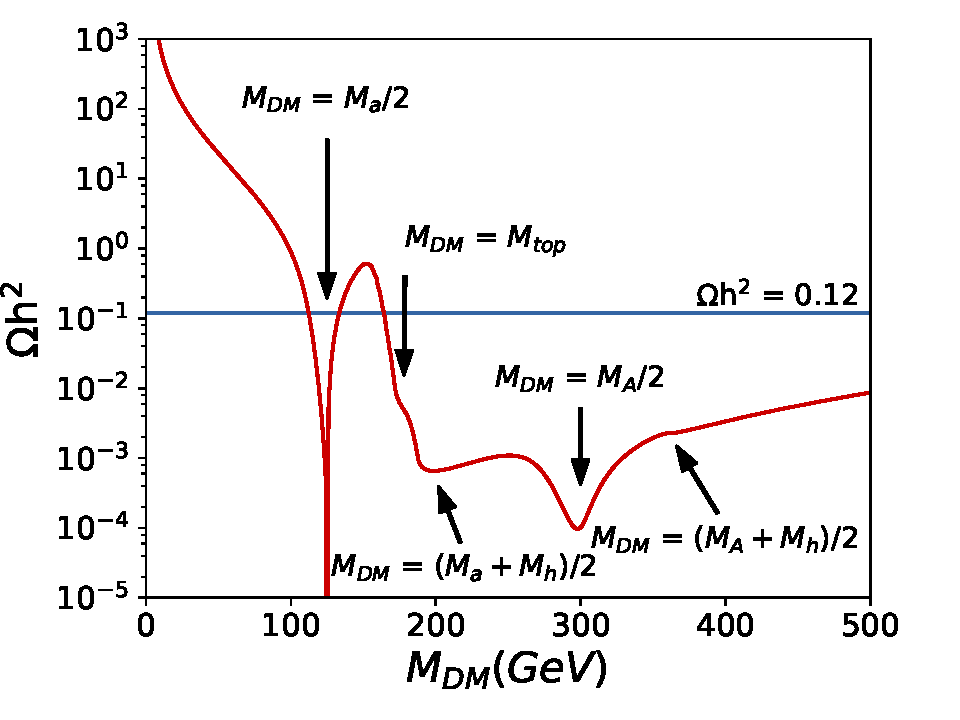
\includegraphics[width=0.8\textwidth]{texinputs/05_relic/figures/relic/line_scan_mdm.pdf}
\caption{Relic density for a one-dimensional scan of \mDM. The other parameters of the model remain fixed with $m_{H}=m_{A}=m_{H^{\pm}}=\unit[600]{GeV}$, $\ma=\unit[250]{GeV}$ and $\tanb=1$, as well as the default choices described in the text. Various kinematic thresholds and regions of resonant enhancement are visible. Consistency with the observed value of $\Omega h^{2} = 0.12$ is mainly controlled by the resonant enhancement of $\chi\chi\rightarrow a$, as well as the onset of $\chi\chi\rightarrow t\overline{t}$.}
\label{fig:relic_scan_mxd}
\end{figure}

The dependence of the relic density on the choice of \mDM is further explored by performing a one-dimensional scan as a function of the DM mass fixing \mH = \mA = $m_{H^{\pm}}$ = 600GeV, \ma = 250GeV, and shown in \autoref{fig:relic_scan_mxd}. 
The relic density confirms structures corresponding to the previously discussed regions of resonant enhancement and to the kinematic boundaries. 
Overall, the behavior is dominated by the low-\mDM suppression of the annihilation cross-section, the resonant enhancement at $\mDM = \ma/2$ and the kinematic top thresholds. 
Other effects, such as the resonant enhancement of $\chi\chi\rightarrow A$ annihilation are present, but only have small effects. 

\begin{figure}[h]
\centering
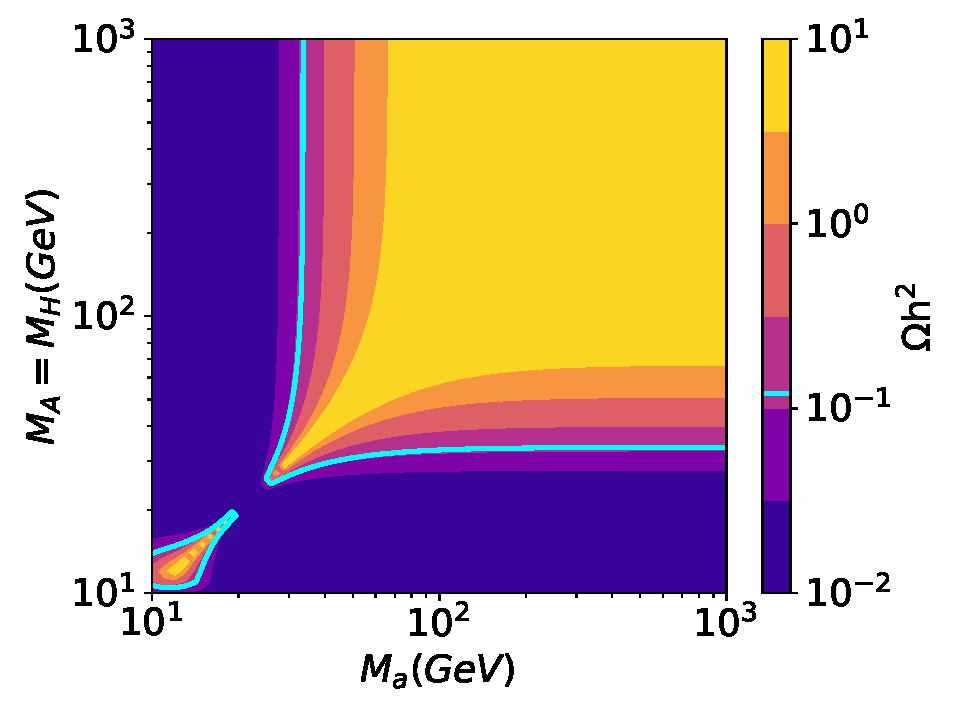
\includegraphics[width=0.49\textwidth]{{texinputs/05_relic/figures/relic/contour_scan_mA_ma_mxd10.pdf}}
\caption{Predicted relic density for a two-dimensional scan of \ma and $\mA=\mH=\mHc$. The other parameters of the model remain fixed with $\mDM=\unit[10]{GeV}$, $\tanb=1$, \mH = \mA = $m_{H^{\pm}}$. The color coding is identical to Fig.~\ref{fig:relic_scan_mxd_ma}.}
\label{fig:relic_scan_mA_ma}
\end{figure}

The relic density values for the \ma-\mA/\mH scan described in \autoref{sec:ParameterScan} is shown in \autoref{fig:relic_scan_mA_ma}. 
For the model parameters chosen in this whitepaper, the regions where the model generates a relic density compatible with the measured value are located at relatively small values of $\ma < \unit[30]{GeV}$ or $\mA=\mH=\mHc < \unit[30]{GeV}$, which are already excluded by LHC and LEP searches (see section 4 of Ref.~\cite{Bauer:2017ota}). 
The cosmological production of DM is largely driven by the choice of $\mDM$. As shown in \autoref{subsub:mDMKinematics}, the model kinematics is largely insensitive to this choice if $\mDM < 2 \ma$. Future experimental results that are sensitive to DM masses around 100 GeV which can yield the measured relic density can still be interpreted by rescaling samples generated according to this parameter scan. 

The $\tanb$-dependent scans, as a function of \ma and \mDM, are shown in Fig.~\ref{fig:relic_scan_mass_tanbeta}. The choice of \tanb acts as an overall modifier of the annihilation cross-section and thus the relic density, and the effect is largely independent of the choice of $\ma$ and $\mDM$. For a choice of $\tanb\approx0.6$, the relic density becomes maximal and steadily decreases for larger and smaller values of \tanb. In the $\mDM$ dependent scan, where \ma is fixed to 250 GeV, the reduction of the relic density at low ($\approx0.1$) and high ($\approx3$) values of $\tanb$ leads to the disappearance of the overabundant island around $\mDM\approx\ma/2$.

\begin{figure}[h]
\centering
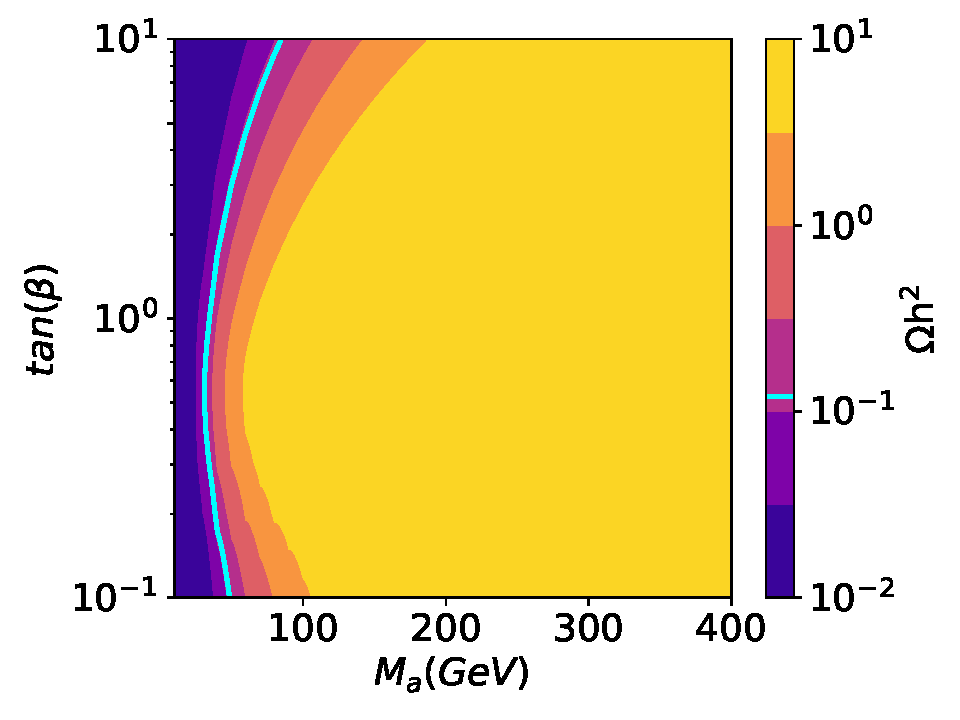
\includegraphics[width=0.49\textwidth]{{texinputs/05_relic/figures/relic/contour_scan_ma_tanbeta.pdf}}
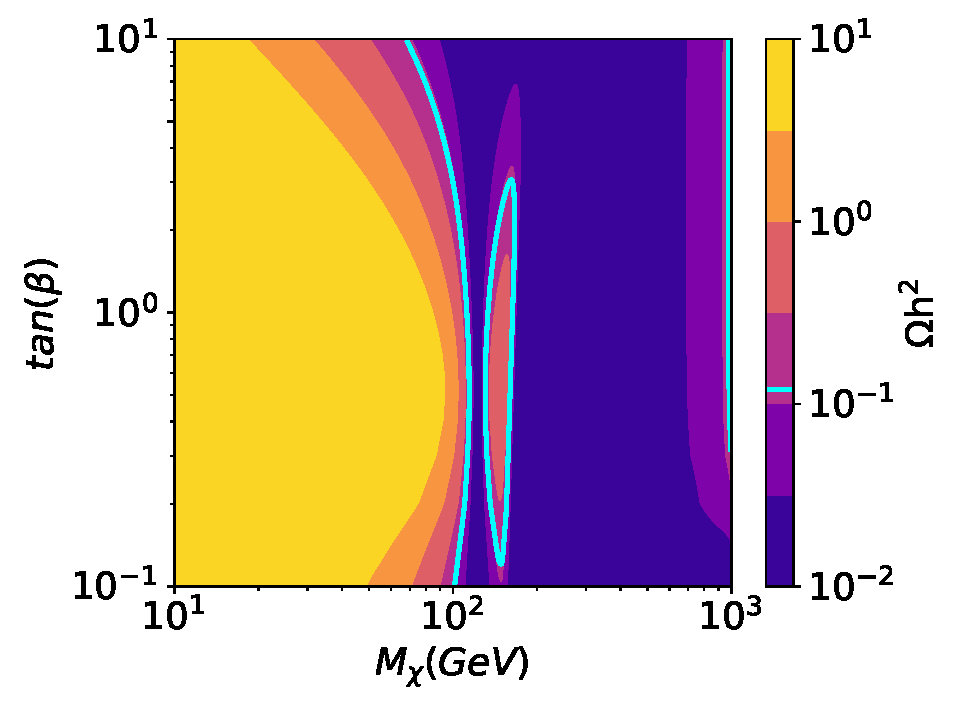
\includegraphics[width=0.49\textwidth]{{texinputs/05_relic/figures/relic/contour_scan_mxd_tanbeta.pdf}}
\caption{Predicted relic density for a two-dimensional scan of \tanb and \ma (left), \mDM (right). In the case of the \mDM ($\ma$) dependent scan, $\ma=\unit[250]{GeV}$ ($\mDM=\unit[10]{GeV}$) is used. The other parameters of the model remain fixed with $m_{H}=m_{A}=m_{H^{\pm}}=\unit[600]{GeV}$, as well as the default choices described in the text. The color coding is identical to Fig.~\ref{fig:relic_scan_mxd_ma}.}
\label{fig:relic_scan_mass_tanbeta}
\end{figure}

%\subsection{Scalar}
%
%\begin{figure}
%    \centering
%    \hspace{2em} 
%    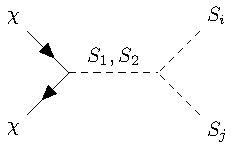
\includegraphics{texinputs/05_relic/figures/relic_scalar/XXSS.pdf} \hspace{3em} \vspace{2em} 
%    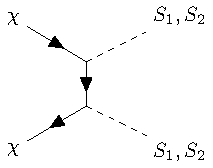
\includegraphics{texinputs/05_relic/figures/relic_scalar/XXSSt.pdf} \hspace{3em} 
%    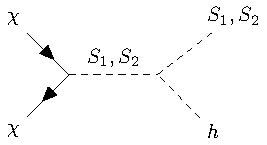
\includegraphics{texinputs/05_relic/figures/relic_scalar/XXSh.pdf}  \hspace{0.5em} \\ 
%    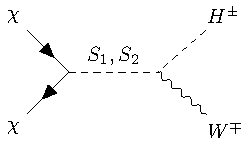
\includegraphics{texinputs/05_relic/figures/relic_scalar/XXWH.pdf} \hspace{2em} 
%    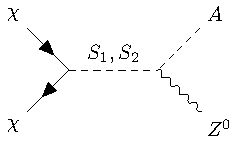
\includegraphics{texinputs/05_relic/figures/relic_scalar/XXZA.pdf} \hspace{2em} 
%    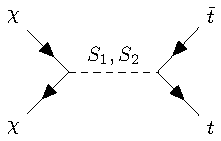
\includegraphics{texinputs/05_relic/figures/relic_scalar/XXtt.pdf} 
%    \caption{Dominant DM annihilation channels, where $(S_i,S_j)$ is one of these scalar final states: $(S_1,S_1)$, $ (S_1,S_2)$, $(S_2,S_2)$, $(H^+,H^-)$, $(A,A)$.}
%    \label{fig:feyn}
%\end{figure}
%
%The 2HDM+S scenario has multiple DM annihilation channels.
%There are tree-level annihilations to fermion-antifermion pairs,
%scalars (the SM Higgs, the two neutral scalars, the pseudoscalar, and the
%charged scalars) and/or the electroweak gauge bosons,
%namely: $\overline{\chi}\chi \rightarrow \overline{f}f$, $S_1 S_1$, $S_2
%S_2$, $S_1 S_2$, $H^+ H^-$, $H^+ W^-$, $A A$, $A Z$, $S_1 h$, and $S_2
%h$ -- these are shown in Fig.~\ref{fig:feyn}. This is to be compared with a single mediator model in which only
%the $\overline{f}f$ and $SS$ channels are present. Note that since all
%diagrams involve $\chi$-scalar vertices (including those with gauge
%boson final states) they are all $p$-wave processes. As such, while we
%will easily be able to find parameters that accommodate the observed
%relic density, there will be no constraints arising from indirect
%detection because the $p$-wave annihilation processes are highly velocity
%suppressed in the late universe.
%
%
%If the DM particle is relatively light, such that annihilation to the
%scalars and electroweak bosons is kinematically forbidden ($m_\chi \lesssim
%80\GeV$), the only annihilation channels that remain open are the
%fermionic ones.  This case is heavily constrained, as the dominant
%annihilation channel is then $b\bar{b}$, which is suppressed by the
%bottom Yukawa coupling and thus usually requires resonant enhancement
%to accommodate the correct relic density.
%
%
%If, instead, the DM particle is heavy enough to annihilate to the Higgs,
%electroweak gauge bosons and/or the new scalars, then these final states will
%likely dominate due to the Yukawa suppression of annihilations to fermions 
%(top excluded).
%Because all of these annihilations are governed by scalar and electroweak
%couplings -- and exist due to gauge invariance, independent of the
%Yukawa couplings of the second doublet -- they are also present,
%for example, in the limit where the second doublet is inert.
%This ability to produce the correct relic abundance independent of
%Yukawa structure means that DM can be adequately produced while
%avoiding any Yukawa dependent constraints (e.g. DD, neutral meson
%mixing, $b \to s \gamma$, $\mu \to e \gamma$, etc.).
%
%%%%%%%%%%%%%%%%%%%%%%%%%%%%%%%%%%%%%%%%%%%
%\begin{figure}[t]
%\centering
%\begin{subfigure}[t]{0.43\textwidth}
%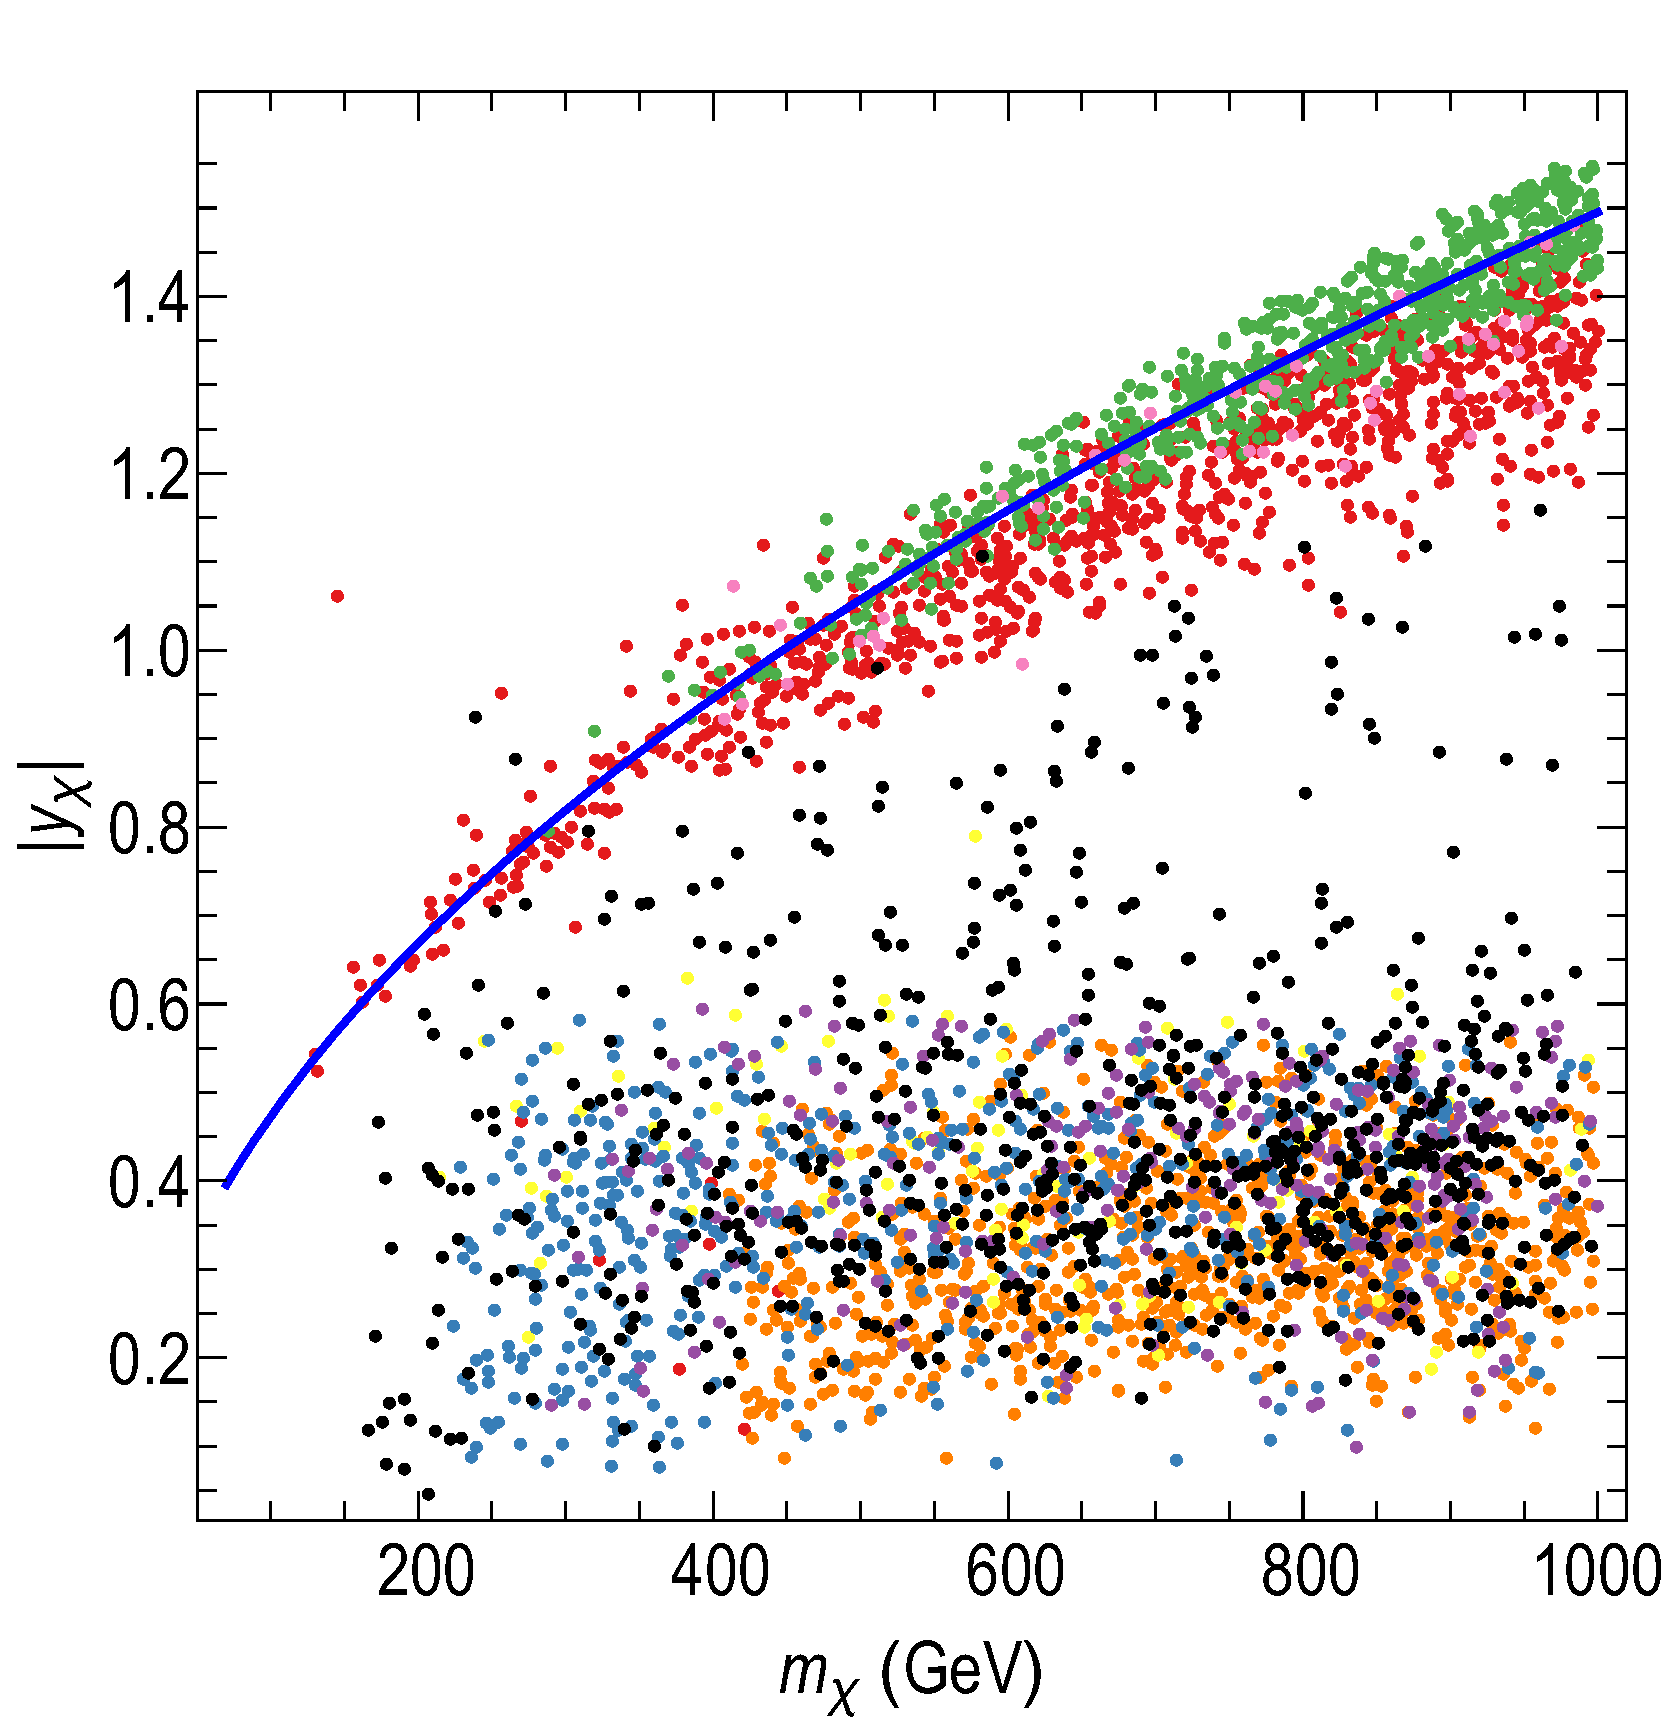
\includegraphics[width=\textwidth]{texinputs/05_relic/figures/relic_scalar/mDM_yDM4.pdf}
%\label{fig:scan1a}
%\end{subfigure}
%\hspace{1em}
%\begin{subfigure}[t]{0.43\textwidth}
%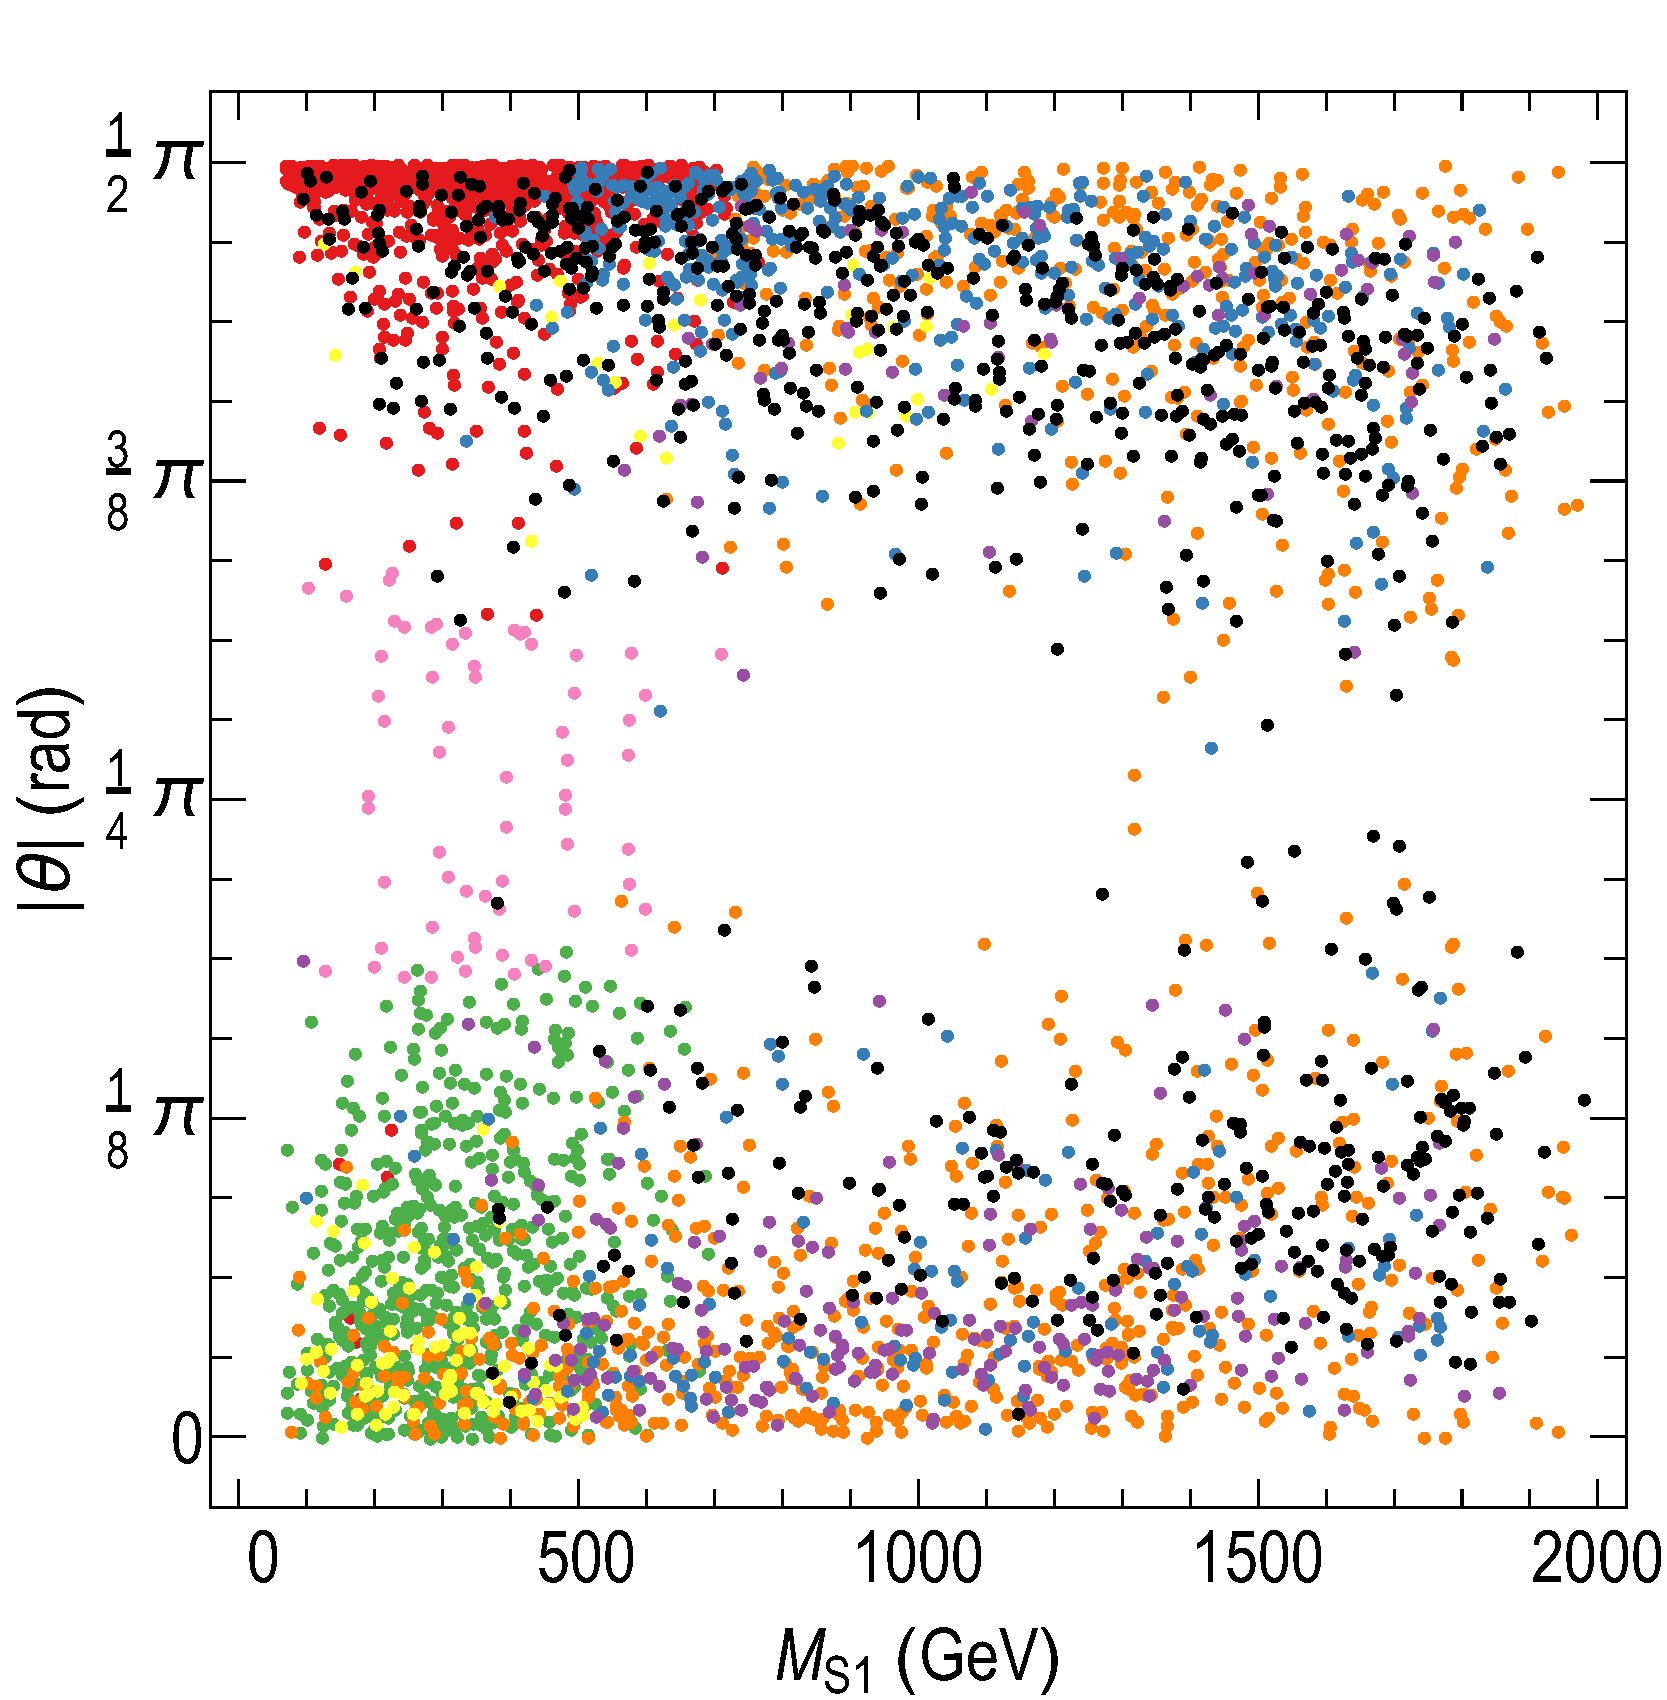
\includegraphics[width=\textwidth]{texinputs/05_relic/figures/relic_scalar/MS1_Theta2.pdf}
%\label{fig:scan1b}
%%\caption{\centering Second Higgs and scalar singlet mixing angle versus DM mass. The plot is symmetric across $| \theta | = \pi / 2$ if extended.}
%\end{subfigure}
%\vspace{0.5ex}
%\begin{subfigure}[t]{0.43\textwidth}
%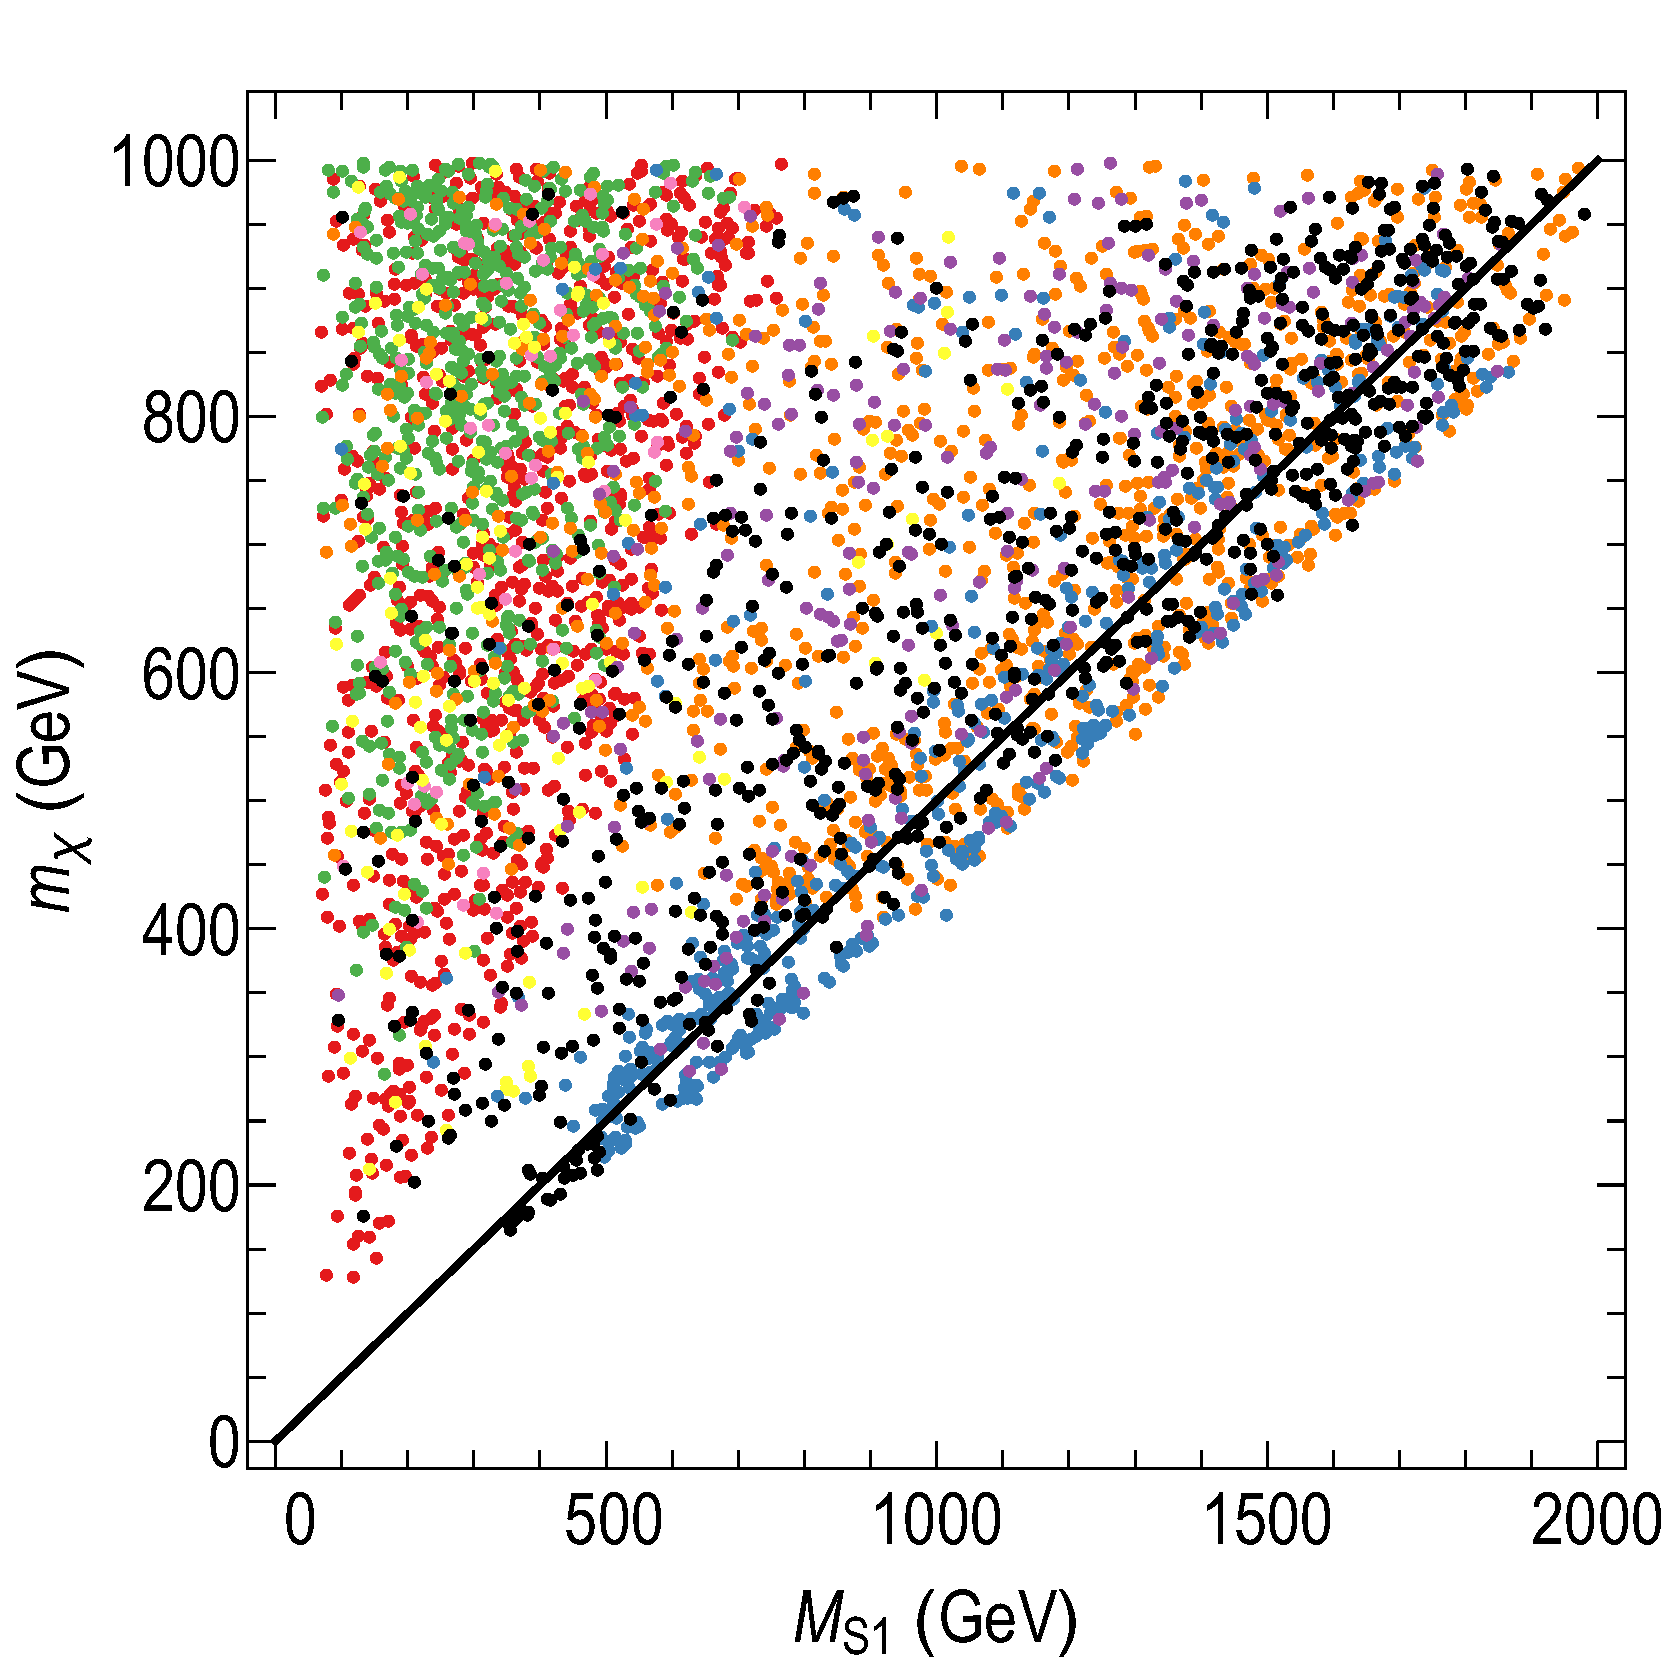
\includegraphics[width=\textwidth]{texinputs/05_relic/figures/relic_scalar/MS1_mDM3.pdf}
%%\caption{DM mass - lighter scalar mass plane $m_\chi - M_{S_1}$.}
%\label{fig:scan1c}
%%\caption{\centering Two additional neutral scalar masses. Note that we have chosen $M_{S_2} > M_{S_1}$; if this is relaxed, then the plot is simply symmetric across the solid black line.}
%\end{subfigure}
%\hspace{1em}
%\begin{subfigure}[t]{0.43\textwidth}
%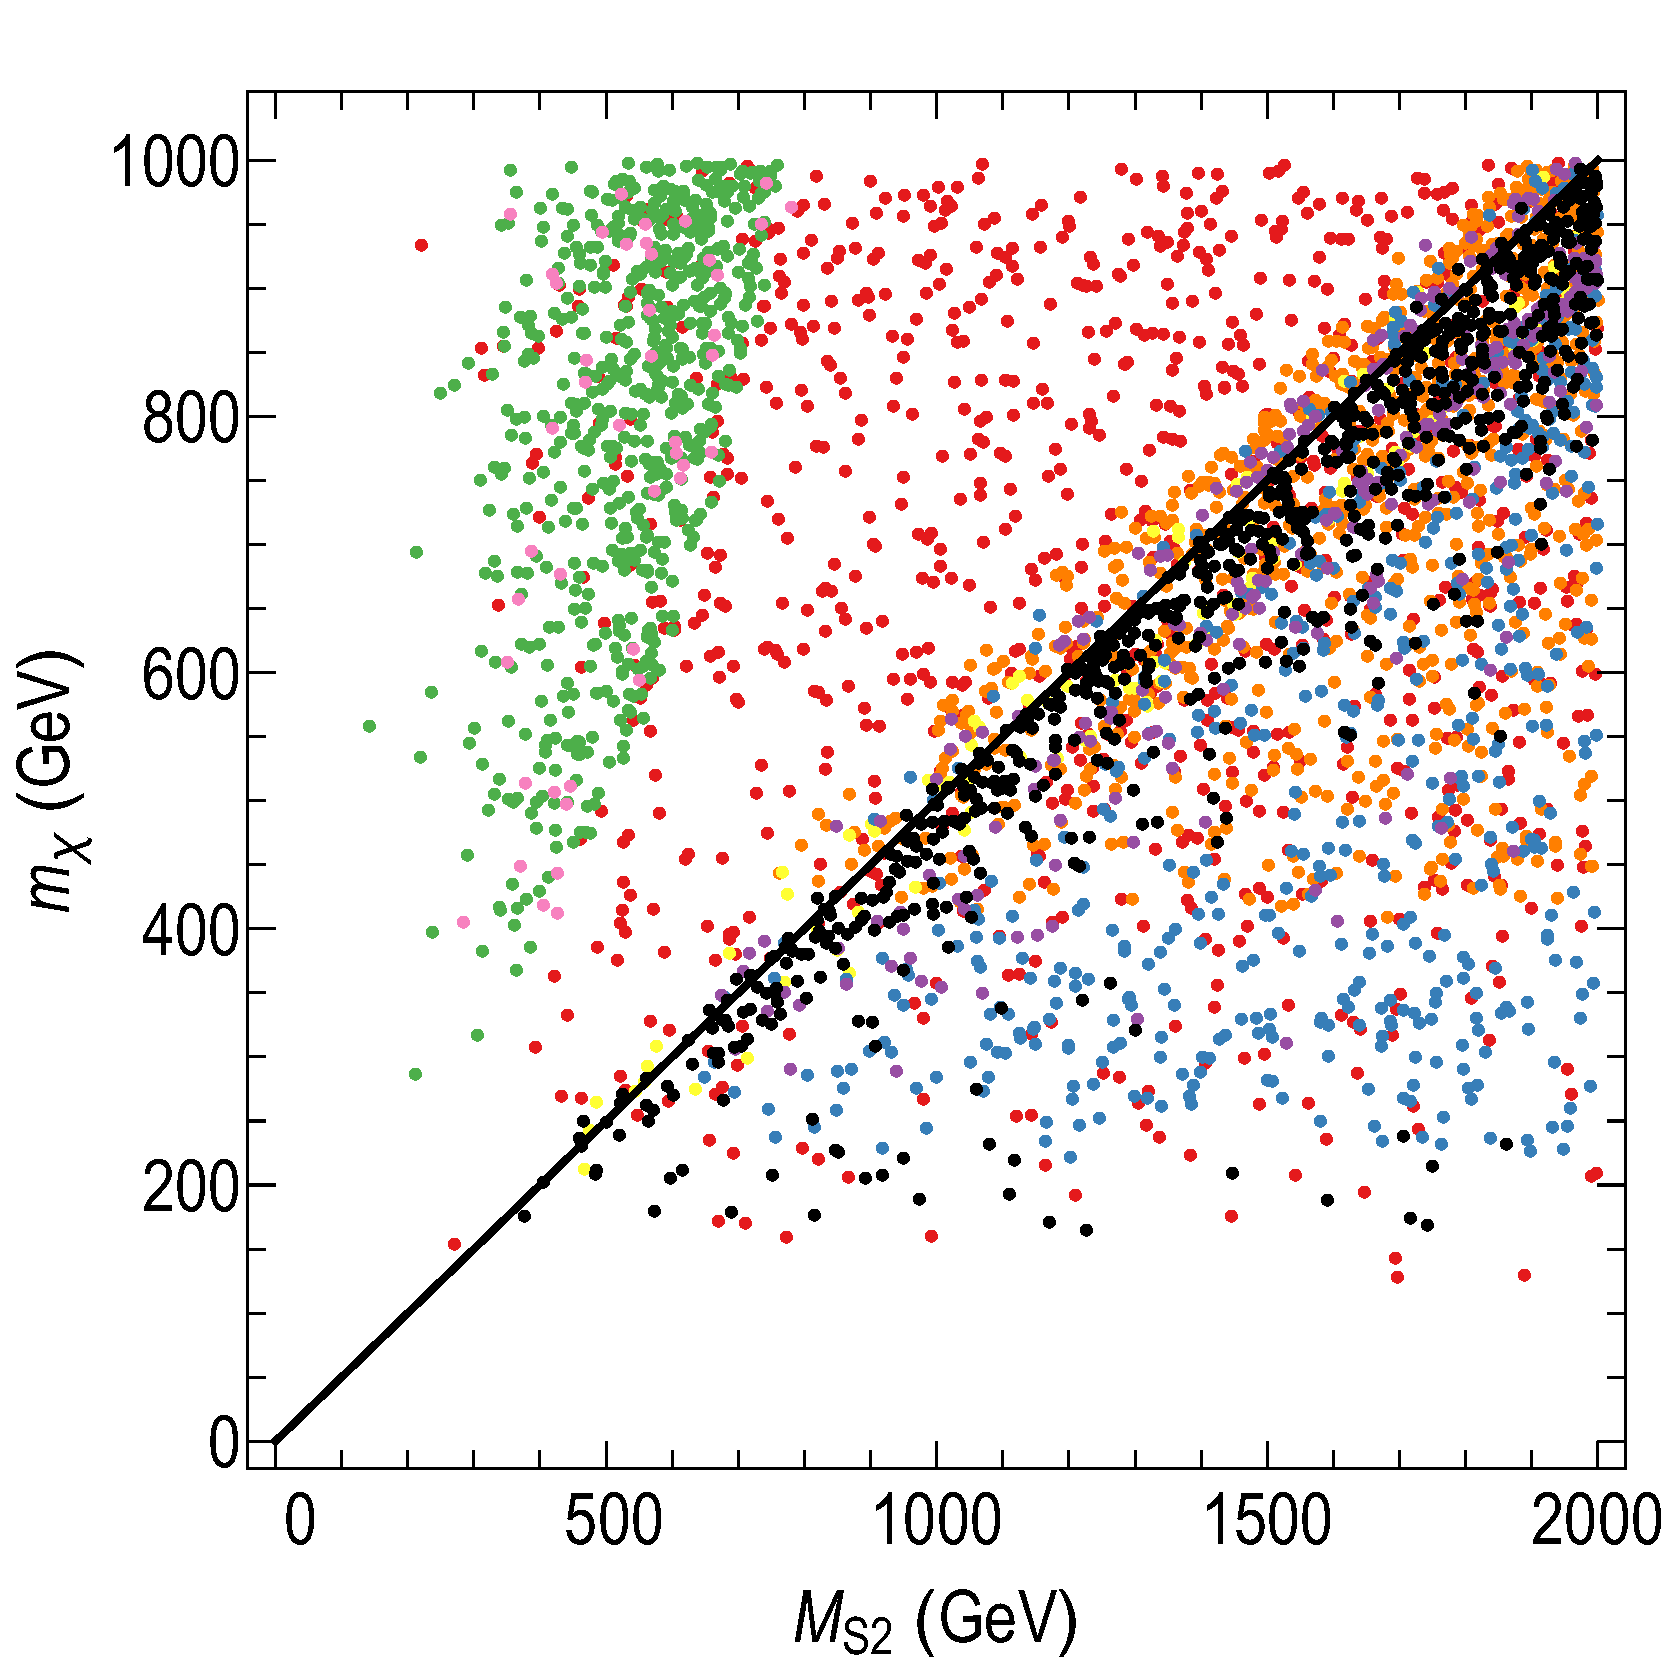
\includegraphics[width=\textwidth]{texinputs/05_relic/figures/relic_scalar/MS2_mDM3.pdf}
%%\caption{DM mass - heavier scalar mass plane $m_\chi - M_{S_2}$.}
%\label{fig:scan1d}
%%\caption{\centering DM mass versus lightest new scalar mass eigenstate.}
%\end{subfigure}\\
%\begin{subfigure}[t]{0.86\textwidth}
%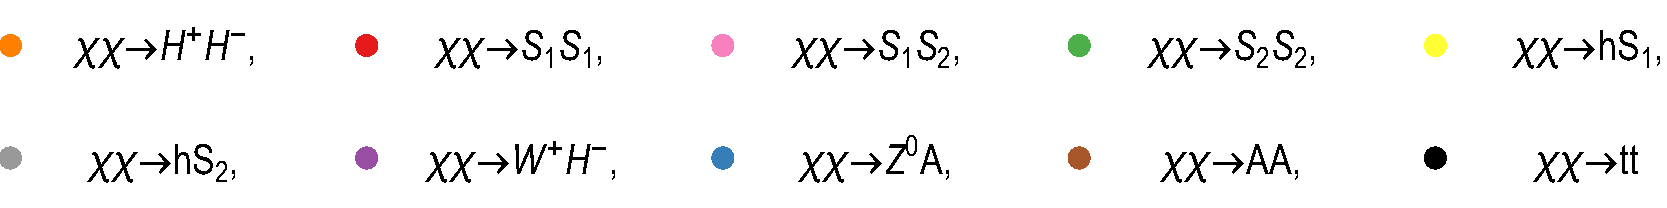
\includegraphics[width=\textwidth]{texinputs/05_relic/figures/relic_scalar/LegendH2.pdf}
%\end{subfigure}
%\caption{Points of our scan of parameter space that produce the correct relic density. The colours represent the dominant annihilation channel, as shown above. 15000 points are taken that survive the constraints, and of them only 25\% of the $H^+H^-$ channel and 10\% of the $S_1S_1$ channel are shown for clarity. The black line in the lower panels indicate $m_\chi = 2 M_{S_1, S_2}$, which is the resonance condition for the s-channel annihilation processes. The blue line in the top left panel represents the scaling expected for a cross section of $\langle \sigma v \rangle \sim y^4_\chi v^2 / 16 \pi^4 m_\chi^2$ which, in this model, applies to a pure $\overline{\chi}\chi \to S_iS_i$ scenario.}
%\label{fig:scan1}
%\end{figure}
%%%%%%%%%%%%%%%%%%%%%%%%%%%%%%%%%%%%%%%%%%%
%
%We implemented the model in Feynrules\footnote{The Feynrules model file used is publicly available in the Feynrules model database.} \citep{Christensen:2008py,Alloul:2013bka} and output the model with the CALCHEP interface~\citep{Christensen:2009jx}. We then used {\tt micrOMEGAs}~\citep{Barducci:2016pcb} to perform the relic density calculation, where we included 3 body final states with off-shell gauge bosons. We also double checked the results by calculating the annihilation cross sections, which are reported in \citep{Bell:2017rgi}. In the case where the parameter values are away from resonances and annihilation thresholds, one can use the wave expansion of the cross sections. The p-wave coefficients of this expansion are also reported in \citep{Bell:2017rgi}.
%
%Sommerfeld enhancement can significantly increase the DM annihilation
%cross section~\citep{Feng:2010zp,Cassel:2009wt,Iengo:2009ni}, provided
%at least one of the scalars is both sufficiently light compared to the
%DM, and strongly coupled to the DM particle.  In practice, for the
%parameter range we consider, this leads to $\mathcal{O}(1)$
%corrections to the cross section; a discussion is provided in
%\citep{Bell:2017rgi}.
%
%%%%%%%%%%%%%%%%%%%%%%%%%%%%%%%%%%%%%%%%%%%
%\begin{figure}[ht]
%\centering
%\begin{subfigure}[t]{0.45\textwidth}
%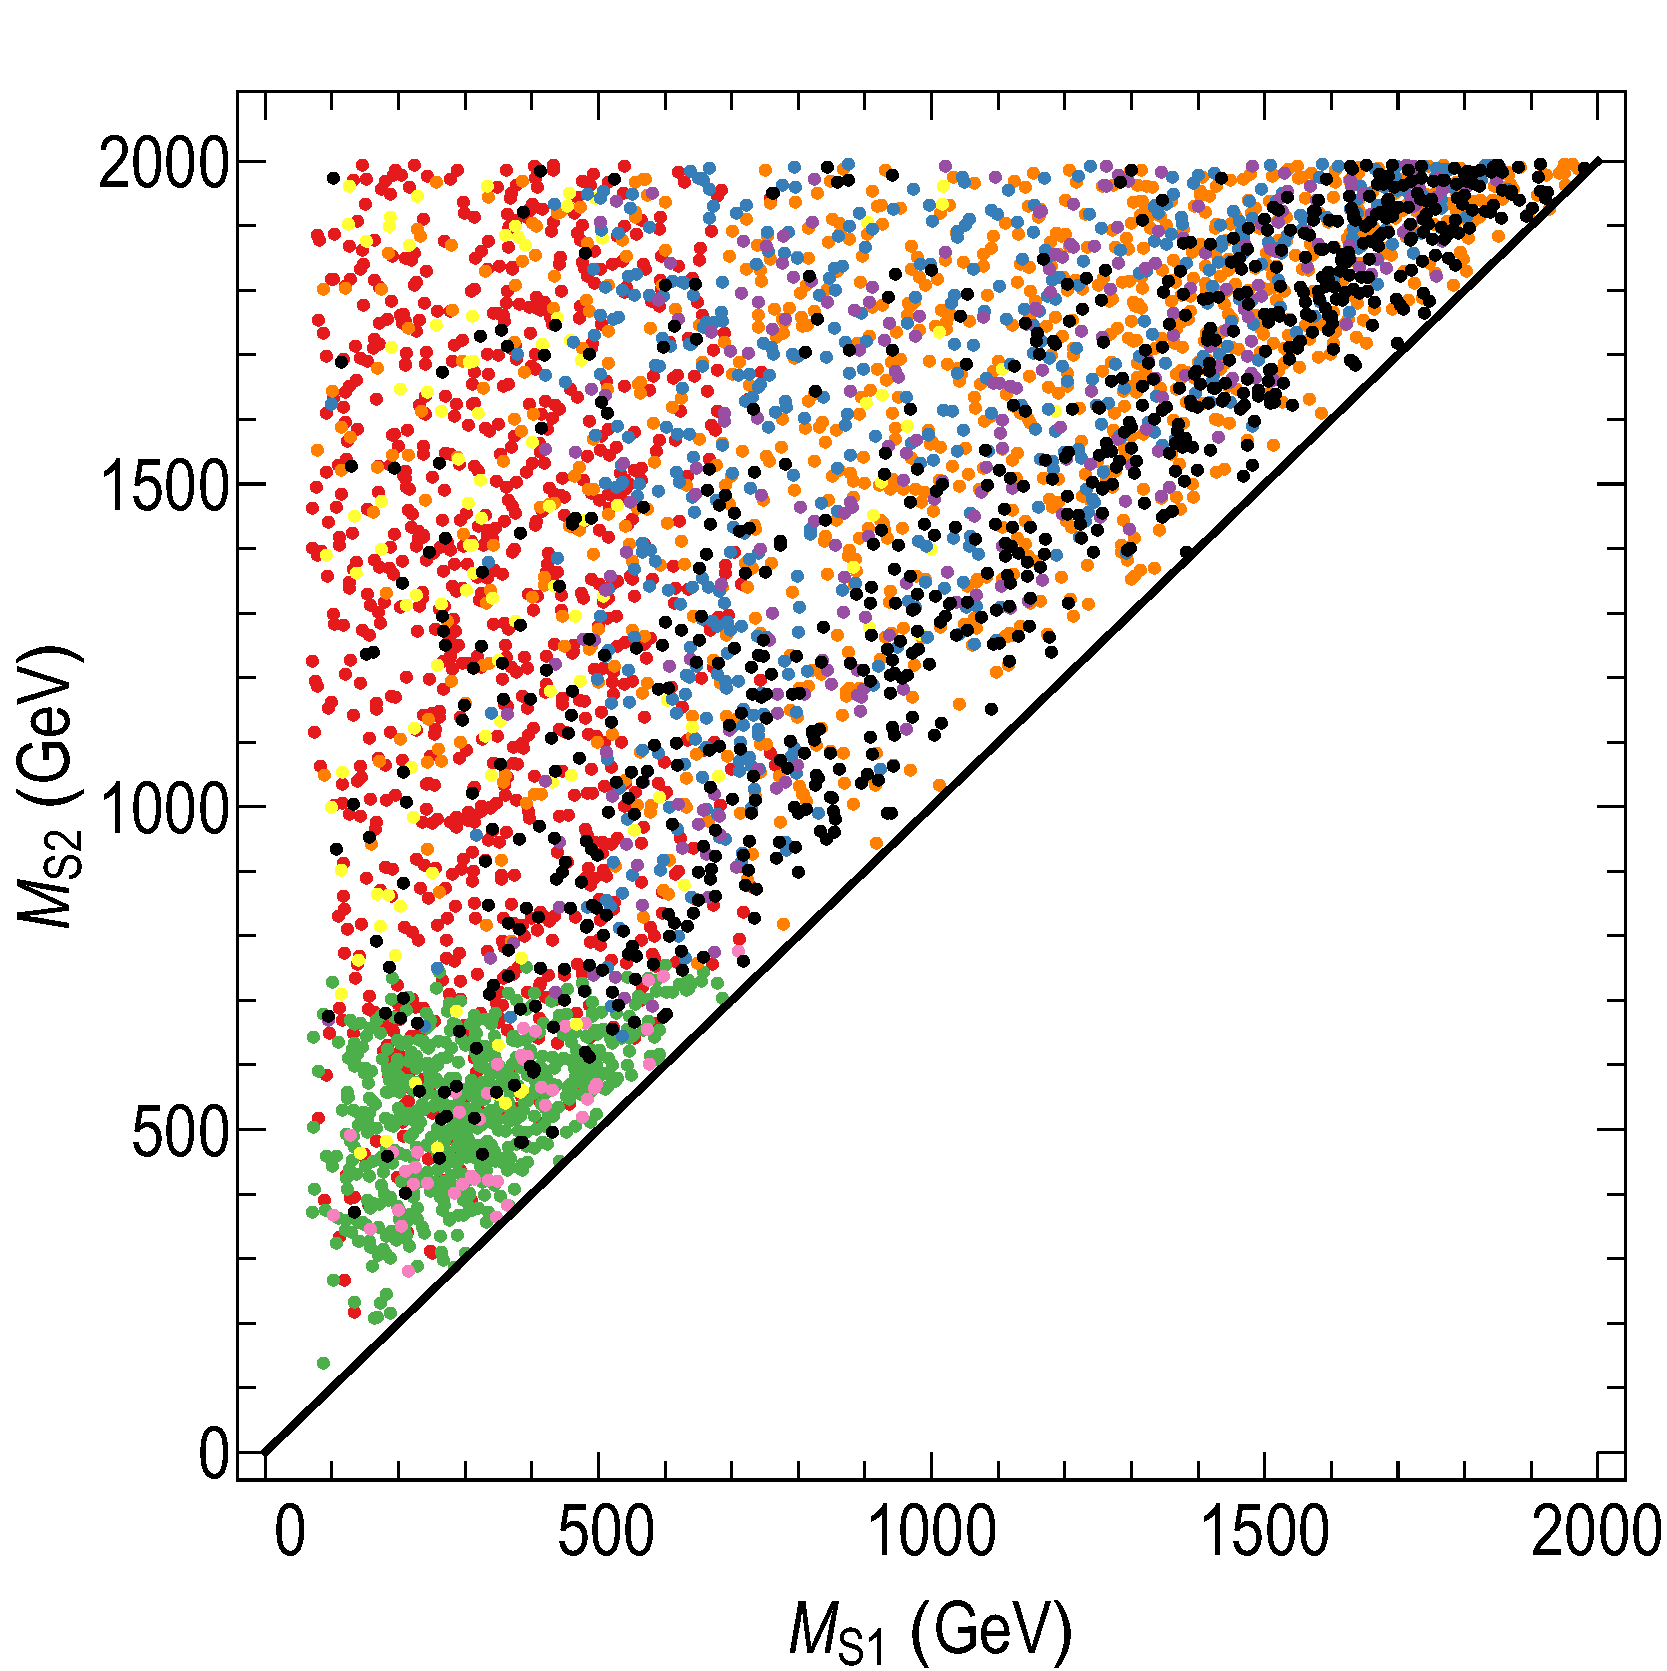
\includegraphics[width=\textwidth]{texinputs/05_relic/figures/relic_scalar/MS1_MS25.pdf}
%%\caption{Heavier - lighter scalar mass plane $M_{S_2} - M_{S_1}$.}
%\label{fig:scan1e}
%%\caption{\centering DM mass versus lightest new scalar mass eigenstate.}
%\end{subfigure}
%\hspace{1em}
%\begin{subfigure}[t]{0.45\textwidth}
%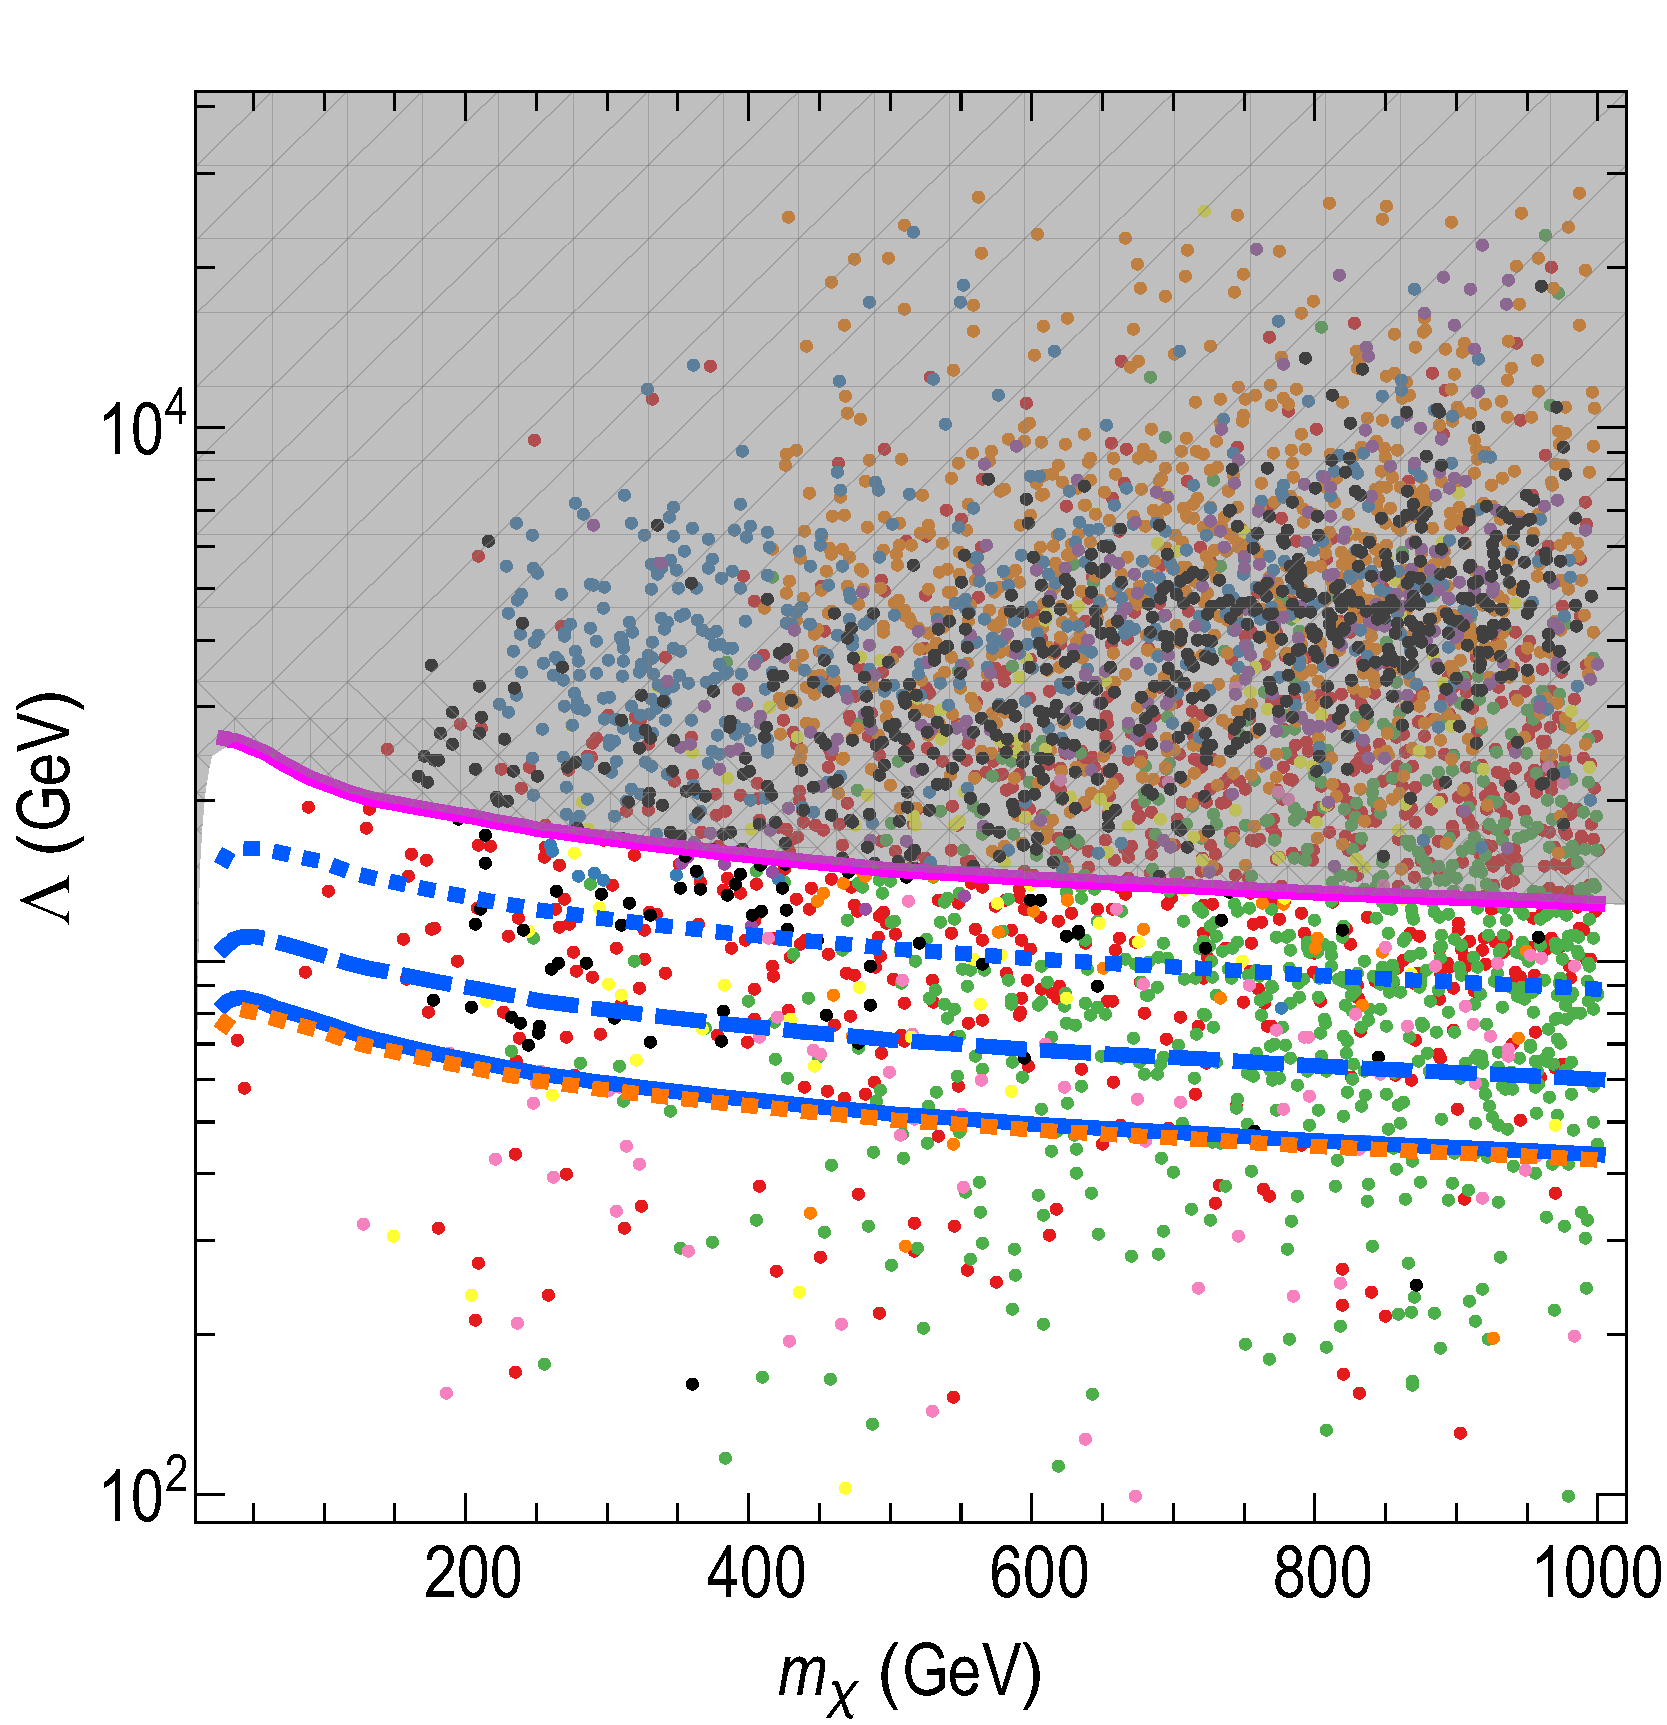
\includegraphics[width=\textwidth]{texinputs/05_relic/figures/relic_scalar/mDM_Lambda4.pdf}
%%\caption{$\Lambda$ versus $m_\chi$}
%\label{fig:scan1f}
%%\caption{\centering DM mass versus lightest new scalar mass eigenstate.}
%\end{subfigure}
%\begin{subfigure}[t]{0.9\textwidth}
%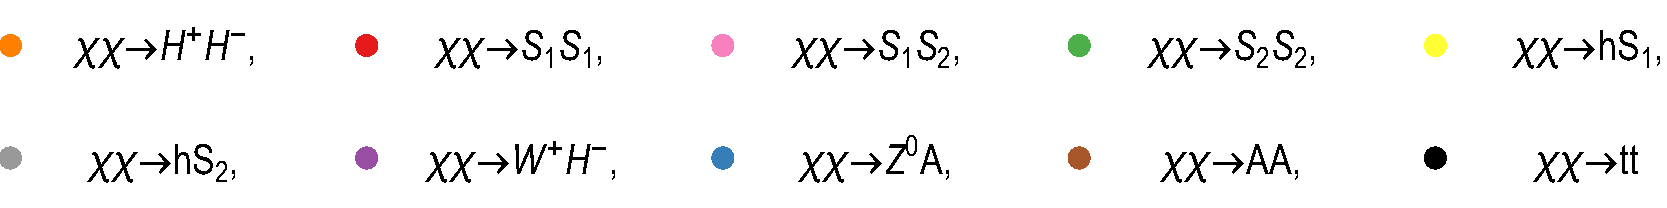
\includegraphics[width=\textwidth]{texinputs/05_relic/figures/relic_scalar/LegendH2.pdf}
%\end{subfigure}
%\caption{Points of our scan of parameter space that produce the correct relic density. The colours represent the dominant annihilation channel, as shown above. 15000 points are taken that survive the constraints, and of them only 25\% of the $H^+H^-$ channel and 10\% of the $S_1S_1$ channel are shown for clarity. $\Lambda$ is the effective cut-off scale for the DD effective operator; the dotted orange line represents the constraint from the LUX 2016 results \citep{Akerib:2016vxi}, the solid blue represents the XENON1T experiment \citep{Aprile:2017iyp}, the dashed blue the projection for the XENON1T experiment with $2t\cdot y$ of data taking, the dotted blue the projection for the XENONnT experiment with $20t\cdot y$ of data taking \citep{Aprile:2015uzo}, and the magenta is the DD sensitivity at the ``neutrino floor''\citep{Billard:2013qya}.}
%\label{fig:scan11}
%\end{figure}
%
%The independent parameters present in the model are
%\be
%m_\chi, \quad M_{S_1}, \quad M_{S_2}, \quad y_\chi, \quad \hat{\lambda}_4, \quad \hat{\lambda}_5, \quad \hat{\lambda}_{hHS}, \quad \hat{\lambda}_{HHS}, \quad \epsilon_u \quad \textrm{and} \quad \epsilon_d.
%\ee
%This set of parameters, through the minima condition and the diagonalization relations, together with the additional constraint $m_\chi = y_\chi v_s$, determine all other parameters of the model\footnote{The phase of the DM Yukawa can always be reabsorbed, so one can chose $y_\chi$ and $v_s$ to be both real and positive.}.
%%
%The scan is performed in the following range:
%\bea
%70\GeV < &m_\chi& < 1\TeV,\\
%70\GeV < &M_{S_1}& < M_{S_2} < 2 \TeV, \\
%0 < &y_\chi& < 2,\\
%&|\hat{\lambda}_{hHS}|& < 2,\\
%&|\hat{\lambda}_{HHS}|& < 4,\\
%0 < &\epsilon_u& < 1,
%\eea
%while for $\hat{\lambda}_4$ and $\hat{\lambda}_5$ we scan over the region shown in \citep{Bell:2017rgi}. 
%These ranges for the couplings were chosen so that most of the points will satisfy unitarity and perturbativity bounds, which was checked via the scalar scattering matrices as in \citep{Bell:2016ekl}.
%To achieve the right relic density, we will see that it will be in general necessary to have $m_\chi\gtrsim M_{S_1}$, and the inequality is strictly required for DM masses below the top mass, as otherwise all considered annihilation channels are closed. In this low DM mass region, however, one needs to take into account Higgs invisible constraints \citep{Aad:2015pla,Khachatryan:2016whc}: 2-body decays forbid the region $2m_\chi<m_h$ and $2M_{S_1}<m_h$, while considering 3-body decays as well further pushes up the lower bound on $M_{S_1}$ to nearly $100\GeV$. The Higgs invisible decays constraints can only be avoided in the $\theta\rightarrow\pi/2$ limit, but in such case the model approaches a decoupled dark sector which is phenomenologically uninteresting\footnote{Relic density requirement can be satisfied in the limit of a decoupled dark sector, in which dark matter annihilates to light dark scalars. However, there would be no signals in collider or direct detection experiments. Moreover, indirect detection is prevented by the p-wave nature of annihilation to scalars, even if small couplings to the SM are included.}. Taking into account these considerations, we have chosen in our scan a conservative lower bound for the DM mass and for the lightest scalar of $70\GeV$.
%Points are selected if they have a relic density between $0.1 < \Omega h^2 < 0.14$ and satisfy all bounds from flavour, unitarity, perturbativity, tree level vacuum stability, and DD constraints. 
%
%\begin{figure}
%\begin{center}
%%\vspace*{1.5cm} 
%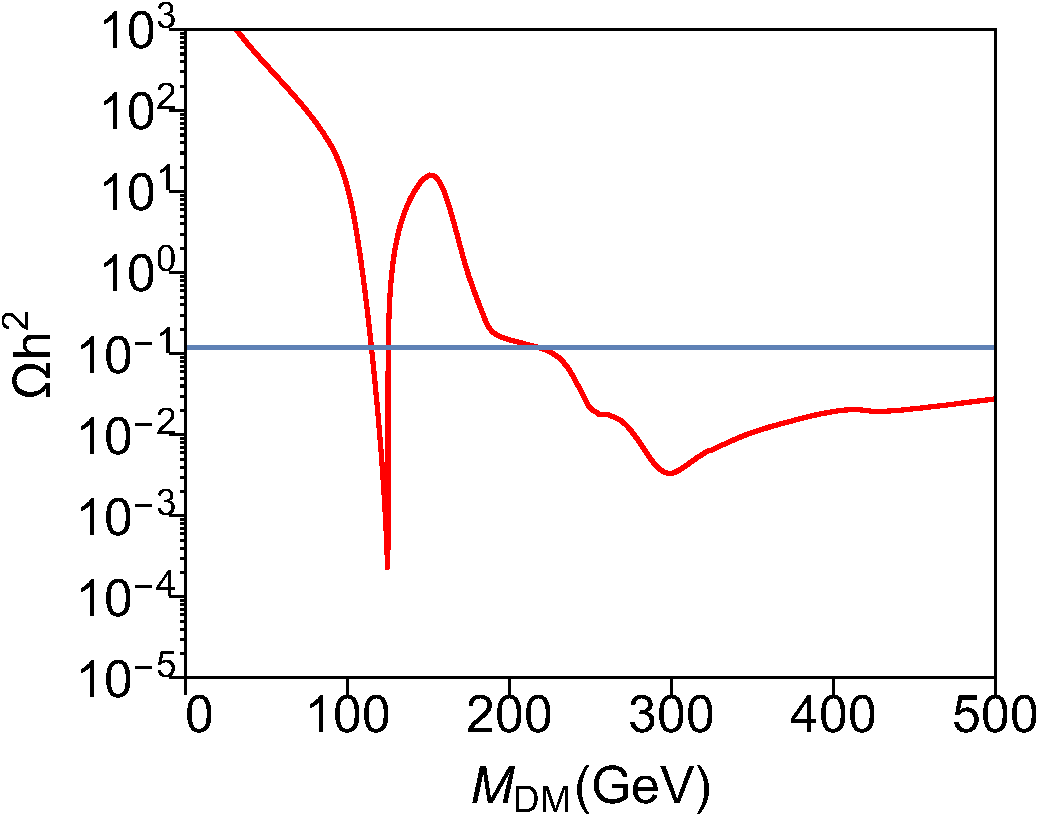
\includegraphics[width=0.7\textwidth]{texinputs/05_relic/figures/relic_scalar/RelicPlot.pdf}
%\caption{One-dimensional scan of the parameter space. We fix all other parameters, see the text for more details.} 
%\label{fig:scalarrelic1D}
%\end{center}
%\end{figure}
%
%The relic density is insensitive to the value of $\epsilon_d$, while the DD results depend on the relationship $\epsilon_d$ and $\epsilon_u$.  
%We set $\epsilon_d = \epsilon_u$ for the scans presented in Fig.~\ref{fig:scan1} and Fig.~\ref{fig:scan11} (with the exception of the right panel of Fig.~\ref{fig:scan11}, which enforces no DD constraint and hence has no $\epsilon_d$ dependence). 
%
%We have chosen to define $S_1$ to be the lighter of the 2 scalars, and allow $\theta$ to range from $0$ to $\pi/2$. As one can always switch the two scalars by sending $\theta\rightarrow\pi/2-\theta$, an equivalent choice would be to take $0<\theta<\pi/4$ without requiring any mass ordering.
%
%In Fig. \ref{fig:scalarrelic1D} we show the value of the relic density obtained through thermal freezeout in a one-dimensional scan, where we kept fixed all parameters except the DM mass. We fix $M_{S_1}=250\GeV$, $M_{S_2}=M_A=M_{H^+}=600\GeV$, $\cos\theta=0.35$ (equivalent to $\sin\theta=0.35$ for the PS model), $y_\chi=1$, 
%
%
%These choices of parameters, along with alignment conditions and $m_\chi = v_s y_\chi$, then fix
%\begin{align}
%    v_s &= \frac{m_\chi}{y_\chi} = m_\chi, \\
%    \lambda_1 &= \frac{m_h^2}{v^2} \sim 0.258, \\
%    \lambda_{s} &= \frac{1}{4 v_s^2} \left( M_{a}^2 + M_A^2 +(M_A^2 - M_a^2) \cos (2\theta ) \right) \sim \frac{222.4^2\GeV^2}{m_\chi^2}, \\
%%    \lambda_{11s} &= 0, \\
%    \lambda_{12s} &= \frac{(M_{S_1}^2 - M_{S_2}^2) \sin (2\theta)}{2 v v_s} \sim -\frac{396.5 \GeV}{m_\chi},\\
%    \lambda_4 &= \frac{1}{2v^2} \left( 2 M_{A}^2 - 4 M_{H^+}^2 + M_{S_1}^2 + M_{S_2}^2 + (M_{S_1}^2 - M_{S_2}^2) \cos (2 \theta ) \right) \sim -0.60, \\
%    \lambda_5 &= -\frac{1}{2v^2} \left( 2 M_{A}^2 - M_{S_1}^2 - M_{S_2}^2 + (M_{S_2}^2 - M_{S_1}^2) \cos (2 \theta ) \right) \sim -0.60, \\
%    \lambda_3 &= \lambda_1 - \lambda_4 - \lambda_5 \sim  1.46.
%\end{align}
%
